\documentclass[notheorems, handout]{beamer}

\usetheme[numbers,totalnumbers,compress, nologo]{Statmod}
\usefonttheme[onlymath]{serif}
\setbeamertemplate{navigation symbols}{}
\setbeamertemplate{theorems}[numbered]
\setbeamertemplate{caption}[numbered]


\mode<handout> {
	\usepackage{pgfpages}
	\setbeameroption{show notes}
	\setbeamercolor{note page}{bg=white}
	\setbeamercolor{note title}{bg=gray!10}
	\setbeamercolor{note date}{fg=gray!10}
}

\setbeameroption{hide notes}

\usepackage[utf8x]{inputenc}
\usepackage[T2A]{fontenc}
\usepackage[russian]{babel}
\usepackage{tikz}
\usepackage{ragged2e}
\usepackage{amsmath,amssymb}
\usepackage{amssymb}   % для \checkmark
\usepackage{pifont}    % для \xmark
\newcommand{\xmark}{\ding{55}}  % определение крестика
\usepackage{graphicx}
\usepackage{caption}
\usepackage{subcaption}
\usepackage{color}
\usepackage{dcolumn}
\usepackage{bm}
\usepackage{float}
\usepackage{csquotes}
\usepackage[backend=biber, style=authoryear, sorting=nyt]{biblatex} % Используем biblatex
\addbibresource{ref.bib} % Имя файла с библиографией
\usepackage{xcolor}

\newtheorem{corollary}{Следствие}
\newtheorem{theorem}{Теорема}
\newtheorem{remark}{Замечание}
\newtheorem{comment}{Замечание}
\newtheorem{lemma}{Лемма}
\newtheorem{sentence}{Предложение}
\newtheorem{definition}{Определение}
\newtheorem{formulation}{Формулировка}
\newtheorem{statement}{Постановка}
\DeclareMathOperator{\R}{\mathbb{R}}
\DeclareMathOperator{\rank}{\mathrm{rank}}
\newcommand{\norm}[1]{\left\|#1\right\|}

\newcommand{\SSA}{\textbf{SSA}}
\newcommand{\EOSSA}{\textbf{EOSSA}}
\newcommand{\GSSA}{\textbf{GSSA}}
\newcommand{\CISSA}{\textbf{CiSSA}}
\newcommand{\TS}{\mathsf{X}}

\newcommand{\MSE}{\operatorname{MSE}}


\title[Модификации метода $\SSA$]{Модификации метода анализа сингулярного спектра для анализа временных рядов: Circulant SSA и Generalized SSA }

\author{Погребников Н. В., гр. 21.Б04-мм}

\institute[Санкт-Петербургский Государственный Университет]{%
	\small
	Санкт-Петербургский государственный университет\\
	Прикладная математика и информатика\\
	Вычислительная стохастика и статистические модели\\
	\vspace{1cm}
%	4 курс (бак.) <<Производственная практика (научно-исследовательская работа)>>\\(Семестр 6)
	Научный руководитель:  д. ф.-м. н., проф. Голяндина Н. Э.
}
	

\date[Зачет]{Санкт-Петербург, 2025}

\subject{Talks}

\begin{document}
\usetikzlibrary{positioning}


\begin{frame}[plain]
	\titlepage

	% \note{Научный руководитель  д.\,ф.-м.\,н., проф. Голяндина Нина Эдуардовна,\\
	% 	кафедра статистического моделирования}
\end{frame}

%\section{Короткая тема}
%\subsection{Общие слова}

%	\setbeameroption{show notes}
\begin{frame}{Структура презентации}
	\textbf{\structure{План доклада:}}
	\begin{enumerate}
		\item \textbf{Введение} — методы, постановка задачи и цели.
		\item \textbf{Критерии сравнения методов}
		\item \textbf{Сравнение SSA и GSSA}
		\item \textbf{Сравнение SSA, разложение Фурье и CiSSA}
		\item \textbf{Итоги и выводы.}
	\end{enumerate}
\end{frame}


\begin{frame}{Введение}
	Пусть $\TS = (x_1, \dots, x_{N})$ -- временной ряд длины \( N \), \( x_i \in \mathbb{R} \) -- наблюдение в момент времени \( i \).

	\(\TS = \TS_{\text{Trend}} + \TS_{\text{Periodics}} + \TS_{\text{Noise}}\), где:
	\begin{itemize}
		\item \( \TS_{\text{Trend}} \) -- тренд, медленно меняющаяся компонента;
		\item \( \TS_{\text{Periodics}} \) -- сумма периодических компонент;
		\item \( \TS_{\text{Noise}} \) -- шум, случайная составляющая.
	\end{itemize}

	\textbf{\structure{Методы}:}
	$\SSA$ -- метод, позволяющий раскладывать временной ряда в сумму интерпретируемых компонент \parencite{golyandina2001analysis};
	$\GSSA$ -- модификация $\SSA$ на основе добавления весов \parencite{gu2024generalized};
	$\CISSA$ -- модификация $\SSA$ на основе циркулярной матрицы \parencite{bogalo2020}.

	\textbf{\structure{Задача}:}
	Описание модификаций в контексте теории $\SSA$, сравнение алгоритмов, реализация их на языке R.

	% \note{
	% 	\textcolor{red}{\textbf{TODO}} Дописать ссылки
	% 	}
\end{frame}

\begin{frame}{Критерии сравнения методов}
	% \textcolor{red}{\textbf{TODO}} Оформить слайд

	{\Large
		\textbf{\structure{Пример}}

		$\TS = \mathsf{S} + \TS_{\mathrm{Noise}}=
			\mathsf{S}^{(1)} + \mathsf{S}^{(2)} + \TS_{\mathrm{Noise}}=
			e^{A{n}}
			\sin\left({2\pi\omega_1 n}\right) +
			\cos\left({2\pi\omega_2 n}\right) + \varepsilon_n$.

		$\omega_1, \omega_2$ -- частоты;
		$\varepsilon_n \sim \mathrm N(0, \sigma^2)$ -- шум;

		$\mathsf{S}$ -- сигнал.

		$\hat{\mathsf{S}}$ -- оценка выделения сигнала методом.

		$\hat{\mathsf{S}}^{(1)},
			\hat{\mathsf{S}}^{(2)}$ -- оценки разделения компонент $\mathsf{S}^{(1)}, \mathsf{S}^{(2)}$.
	}


	\bigskip

	\textbf{\structure{Критерии сравнения методов:}}
	\begin{itemize}
		\item Выделение сигнала;
		\item Разделимость;
		\item Постановка задачи (для CiSSA частоты предполагаются известными).
	\end{itemize}

\end{frame}


\begin{frame}{Разделимость}
	% $\mathrm M(\TS_N; \Theta)$ -- разделения ряда на компоненты с параметрами \( \Theta \). 
	\( \TS_N = \TS^{(1)}_N + \TS^{(2)}_N \).
	$\mathrm M$ -- метод разделения ряда на компоненты с параметрами $\Theta$.
	$\hat{\TS}_N^{(1)}$ -- оценка $\TS_N^{(1)}$, восстановленная $\mathrm M$.
	\begin{definition}
		\label{def:exact}
		Ряды \( \TS^{(1)}_N \) и \( \TS^{(2)}_N \) точно разделимы методом $\mathrm M$, если существует такое \( {\Theta} \), что \( \mathrm{MSE}\left(\TS^{(1)}_N, \hat{\TS}^{(1)}_N\right) = 0 \).
	\end{definition}

	\begin{definition}
		\label{def:asymp}
		Ряды \( \TS^{(1)}_N \) и \( \TS^{(2)}_N \) асимптотически разделимы методом $\mathrm M$, если существует последовательность \( {\Theta}(N)\), \( N \rightarrow \infty \), что \( \mathrm{MSE}\left(\TS^{(1)}_N, \hat{\TS}^{(1)}_N\right) \rightarrow 0 \).
	\end{definition}

	\note{Какое из оформлений лучше?}
\end{frame}



\begin{frame}{Метод SSA. Алгоритм}
	\( \TS = (x_1, \ldots, x_N) \) — временной ряд.  \( 1 < L < N \) --  длина окна.
	\textbf{\structure{Алгоритм $\SSA$}}:

	\begin{enumerate}
		\item \textbf{Построение траекторной матрицы:}

		      $
			      \mathbf X = \mathcal{T}_L(\TS) = [\TS_1 : \ldots : \TS_K], \, \TS_i = (x_i, \ldots, x_{i+L-1})^T, \,$

		      $
			      1 \leq i \leq K, \quad K = N - L + 1.
		      $

		\item \textbf{Сингулярное разложение (SVD)}  траекторной матрицы.
		\item \textbf{Группировка} элементарных матриц SVD.
		\item \textbf{Восстановление} временного ряда по матрицам SVD:

		      $\TS = \tilde \TS_{1}  + \dots + \tilde \TS_{m}$.
	\end{enumerate}
	\note{Какое из оформлений лучше?}
\end{frame}


\begin{frame}{Вложенный вариант SSA. EOSSA}
	% \textcolor{red}{\textbf{TODO}} Указать, что такое вложенный вариант, сказать, что таким образом улучшается разделимость. Так получается лучше разделять компоненты между собой
	$\TS = \mathsf{S} + \TS_{\mathrm{Noise}}=
		\mathsf{S}^{(1)} + \mathsf{S}^{(2)} + \TS_{\mathrm{Noise}}$


	\begin{definition}[\cite{Golyandina_2015}]
		\textbf{Вложенный вариант SSA} — двухэтапный метод:
		\begin{enumerate}
			\item Задается $r$. $\tilde {\mathbf{S}}$ -- сумма первых $r$ слагаемых SVD разложения траекторной матрицы сигнала $\mathbf S$ с помощью базового $\SSA$ .
			\item Применение другого метода к $\tilde{\mathbf{S}}$ для улучшения разделимости: $\tilde{\mathbf{S }} = \tilde{\mathbf{S}}_1 + \tilde{\mathbf{S } }_2$.
		\end{enumerate}
	\end{definition}
	\bigskip
	$\SSA$ $\EOSSA$ \parencite{golyandina2023intelligent} является вложенным вариантом $\SSA$.
\end{frame}



\begin{frame}{Метод GSSA. Алгоритм}
	\( \TS = (x_1, \ldots, x_N) \) — временной ряд,  параметры \(L\) и  $\alpha \geq 0$.

	$	{\boldsymbol{w}}^{(a)} = (w_{1}, w_{2}, \ldots, w_{L}) = \left( \left| \sin\left(\frac{\pi n}{L+1}\right) \right|^\alpha \right),  \quad n = 1, 2, \dots, L$.


	\bigskip

	\textbf{\structure{Шаг 1 алгорима $\GSSA$}}:

	$\mathbf{X}^{(\alpha)} = \mathcal{T}_L^{(\alpha)}(\TS) = [\TS_1^{(\alpha)} : \ldots : \TS_K^{(\alpha)}]$,
	$\TS_i^{(\alpha)} = ( w_1 x_{i-1}, \ldots, w_L x_{i+L-2})^{\mathrm{T}}$,
	$1 \leq i \leq K$.

	\medskip

	\textbf{\structure{Шаги 2-4}}: аналогичны $\SSA$.

	\bigskip

	\begin{comment}
	При $\alpha = 0$, $\GSSA$ --- в точности базовый алгоритм $\SSA$.
	\end{comment}

	\medskip

	\begin{comment}
	${\boldsymbol{w}}^{(a)}$ называются степенными синусными весами. Они могут иметь другой вид.
	\end{comment}


	% \note{
	% 	\textcolor{red}{\textbf{TODO}} 
	% 	Сослаться на статью авторов.
	% 	}
\end{frame}


\begin{frame}{Сравнение SSA и GSSA. Линейные фильтры 1}

	\begin{definition}
		Пусть $\TS = (\dots, x_{-1}, x_0, x_1, \dots)$ — бесконечный временной ряд.

		\textbf{Линейный конечный фильтр} — оператор $\Phi$, преобразующий $\TS$ в $\mathsf{Y} = (\dots, y_{-1}, y_0, y_1, \dots)$ по правилу:
		\begin{equation*}
			y_j = \sum_{i = -r_1}^{r_2} h_i x_{j-i}, \quad j \in \mathbb{Z},
		\end{equation*}
		где $r_1 + r_2 + 1$ — ширина фильтра, $h_i \in \mathbb{R}$ — коэффициенты.
	\end{definition}

	\textbf{\structure{Пример.}} При применении фильтра $\Phi$ к $x_j = \cos{2\pi \omega j}$, получается ряд
	$y_j = A_{\Phi}(\omega) \cos\left(2\pi\omega j + \phi_{\Phi}(\omega) \right)$.

	$\phi_{\Phi}(\omega)$ -- фазово-частотная характеристика (ФЧХ).

	$A_{\Phi}(\omega)$ -- амплитудно-частотная характеристика (АЧХ).
\end{frame}

\begin{frame}{Сравнение SSA и GSSA. Линейные фильтры 2}
	$\TS = (x_1, \dots, x_{N})$, $(\sqrt{\lambda},\,U,\,V)$ -- собственная тройка $\SSA$. $U = (u_1, \dots, u_L)$.
	$\widetilde \TS = \mathcal{T}_L \circ \mathcal{H} ( \sqrt{\lambda} U V^T )$.

	\textbf{\structure{Запись $\SSA$ через линейный фильтр для средних точек}}:
	\begin{equation*}
		\label{eq:representation_ssa_as_filter}
		{\widetilde{x}}_{s} = \sum_{j=-(L-1)}^{L-1} \left( \sum_{k=1}^{L-|j|} u_{k} u_{k+|j|} / L \right) x_{s-j}, \quad L \leq s \leq K.
	\end{equation*}

	\textbf{\structure{Аналогичное представление для $\GSSA$}}:
	\begin{equation*}
		\label{eq:representation_gssa_as_filter}
		{\widetilde{x}}_{s} = \sum_{j=-(L-1)}^{L-1} \left( \sum_{k=1}^{L-|j|} u_{k}^{(\alpha)} u_{k+|j|}^{(\alpha)} w_k / \sum\limits_{i = 1}^{L}w_i \right) x_{s-j}, \quad L \leq s \leq K.
	\end{equation*}

	\begin{remark}
		Представление через линейные фильтры можно получить и для остальных точек ряда.
	\end{remark}

	% \note{
	% \textcolor{red}{\textbf{TODO}} 
	% Убрать весь текст, оставить только представление в виде фильтров 
	% }
\end{frame}


\begin{frame}{Сравнение SSA и GSSA. Пример}
	$\TS = \TS_{\sin} + \TS_{\cos} = \sin\left(\frac{2\pi}{12} n \right) + \frac{1}{2}\cos\left(\frac{2\pi}{19} n \right)$. $N = 96 \cdot 2 - 1$, $L = 48$.

	Группировка: для $\TS_{\sin}$ 1-2 SVD, для $\TS_{\cos}$ 3-4 SVD.

	\begin{figure}[ht]
		\centering
		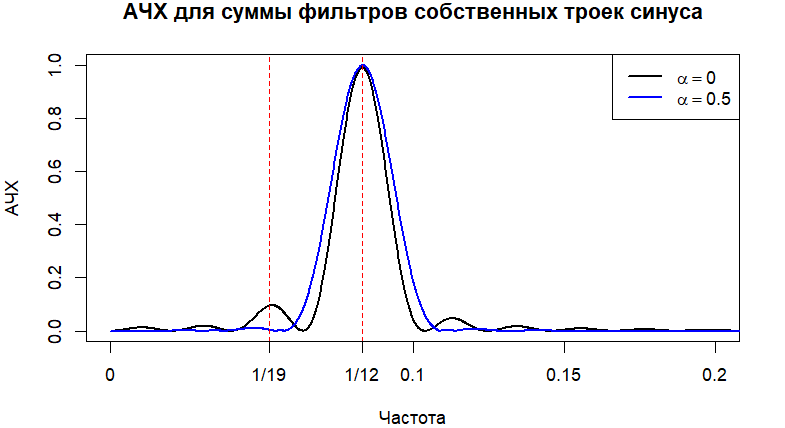
\includegraphics[width=0.8\textwidth]{../Text/img/various_alphas_sin_cos.png}
		\label{fig:various_alphas_sin_cos}
	\end{figure}
	\(\alpha = 0.5\): шире полоса пропускания фильтра, чем при $\alpha = 0 $, но нет волнообразного поведения на краях.
\end{frame}

\begin{frame}{Сравнение SSA и GSSA. Пример продолжение}
	\begin{figure}[ht]
		\centering
		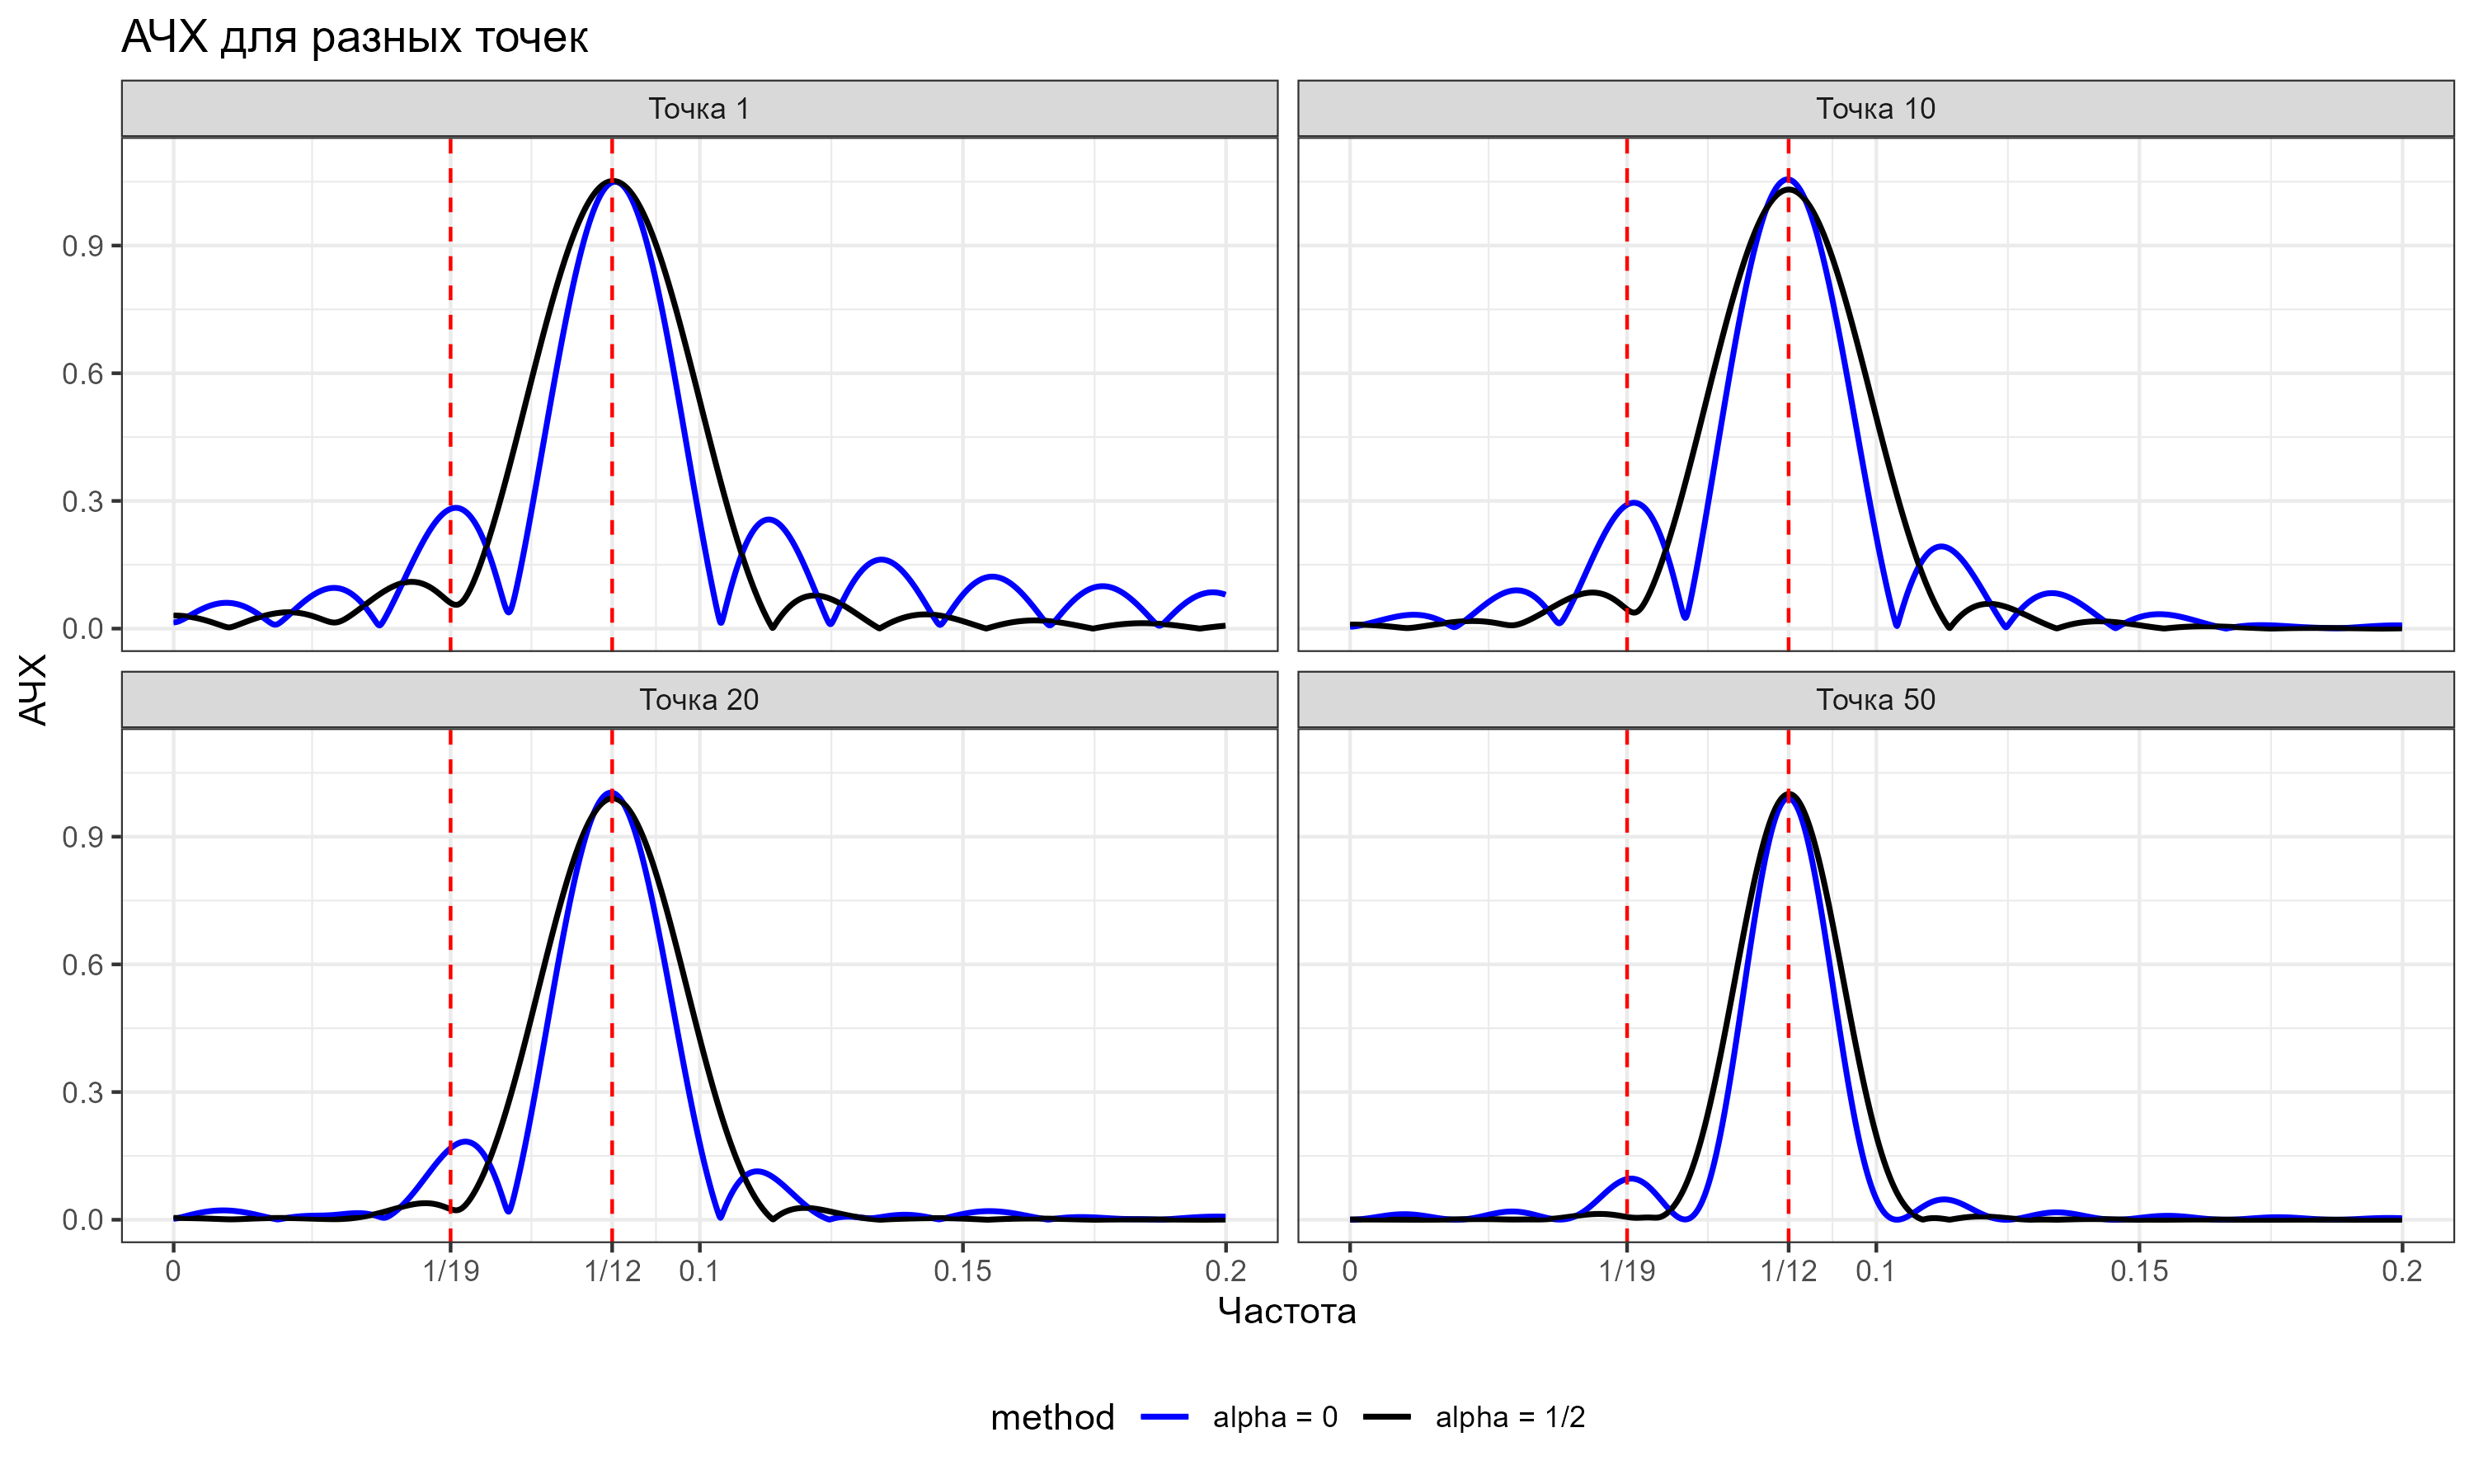
\includegraphics[width=0.95\textwidth]{img/trend inseparability example/afc_4_points.png}
	\end{figure}
	Таким образом, АЧХ фильтра также зависит от точки, для которой этот фильтр построен.
\end{frame}

\begin{frame}{Сравнение SSA и GSSA. Пример продолжение 2}
	\begin{figure}[ht]
		\centering
		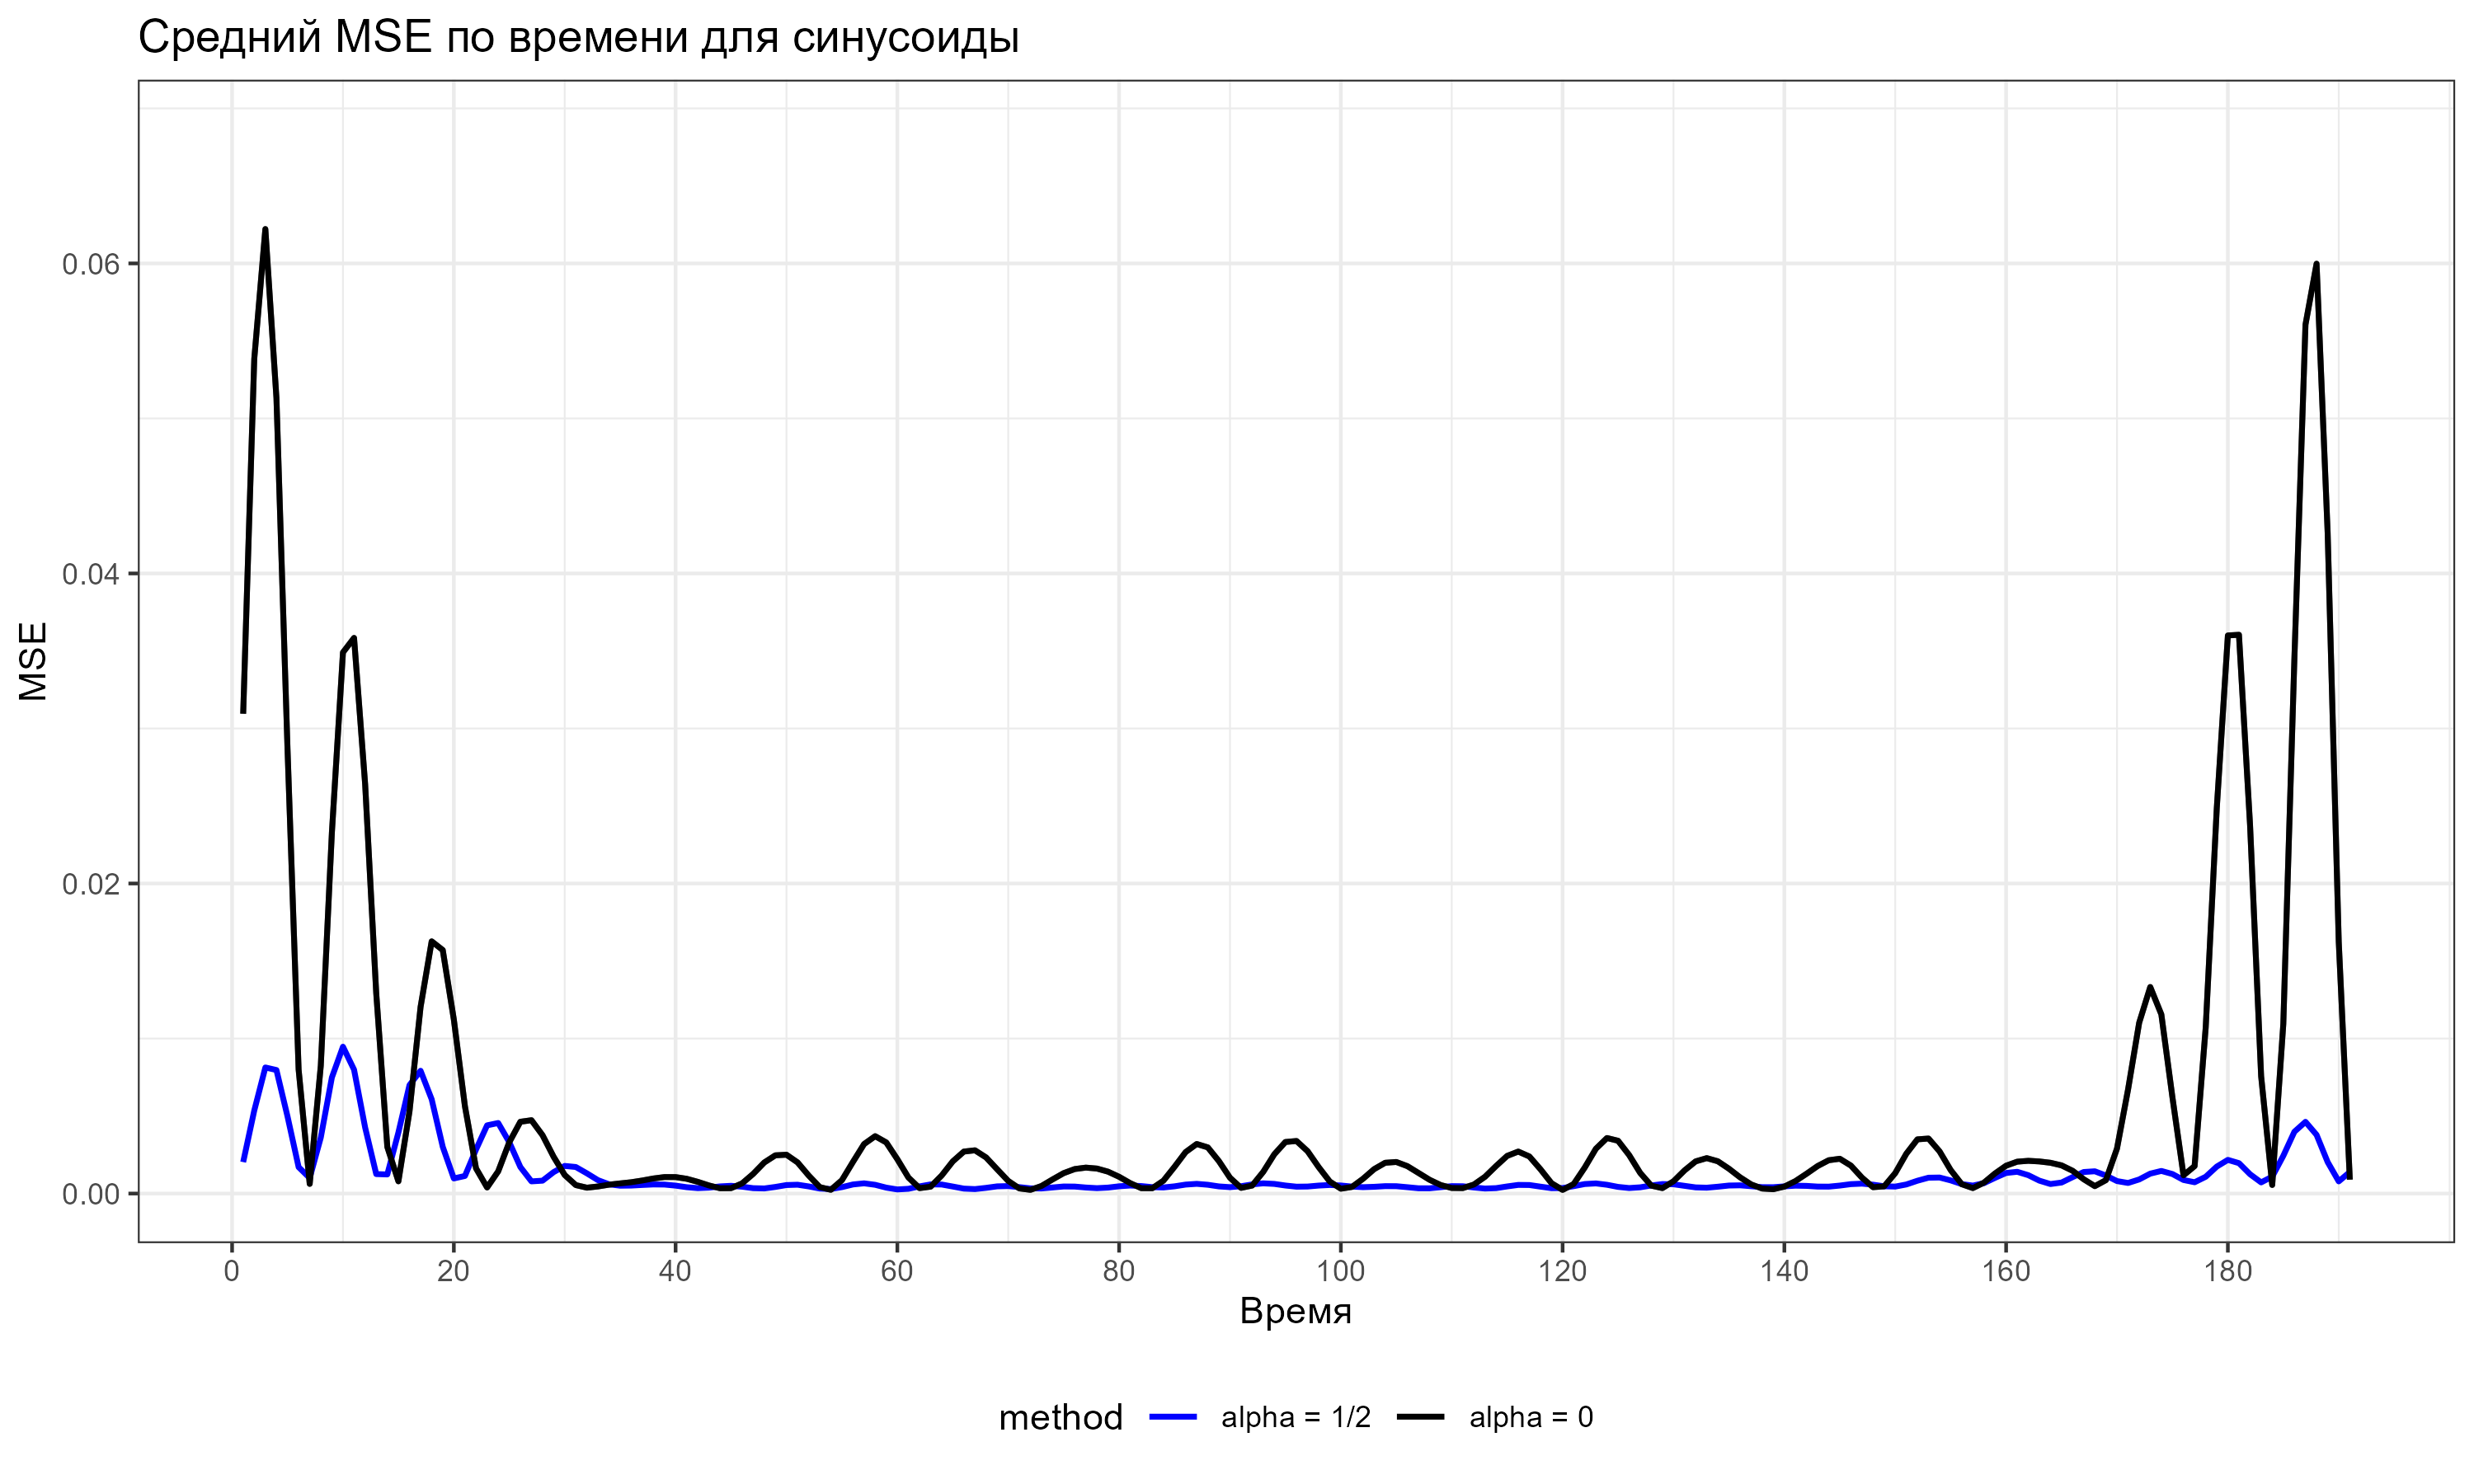
\includegraphics[width=0.95\textwidth]{img/trend inseparability example/mse_y1_time.png}
	\end{figure}
	В начальных и конечных значениях ошибки больше.
\end{frame}


\begin{frame}{Вывод. Вложенный вариант SSA + GSSA}
	\begin{table}[H]
		\label{tab:errs_ssa_gssa_united}
		\centering
		\caption{$\TS_{\sin} + \TS_{\cos}+
				\varepsilon_n$, $\varepsilon_n \sim \mathrm N(0, 0.1^2)$, MSE оценок }
		\begin{tabular}{l|ccc}
			\hline
			Метод/Ошибка                     & $\TS_{\sin}$      & $\TS_{\cos}$      & $\TS$             \\
			\hline
			$\SSA$                           & 5.68e-03          & 5.44e-03          & \textbf{7.48e-04} \\
			$\GSSA$, $\alpha = 0.5$          & \textbf{1.21e-03} & \textbf{1.25e-03} & 1.04e-03          \\
			\hline
			$\SSA$ + $\GSSA$, $\alpha = 0.5$ & \textbf{1.06e-03} & \textbf{1.12e-03} & \textbf{7.15e-04} \\
			\hline
		\end{tabular}
	\end{table}

	Получается вложенный вариант $\SSA$.

	% \textcolor{red}{\textbf{TODO}} 
	% Дописать, что получился вложенный вариант алгоритма.
\end{frame}





\begin{frame}{Метод CiSSA. Алгоритм}
	\( \TS = (x_1, \ldots, x_N) \) — временной ряд.  \( 1 < L < N \) --  длина окна.
	\textbf{\structure{Алгоритм $\CISSA$}}:
	\begin{enumerate}
		\item \textbf{Построение траекторной матрицы:} как в $\SSA$.

		\item $l = 1:L$, ${U}_{l}=L^{-1/2}(u_{l,1},\dots,u_{l,L}), \, u_{l,j}=\exp\left(-\mathrm{i}2\pi(j-1)\frac{l-1}{L}\right).$
		      \textbf{Элементарное разложение:} $\omega_k = \frac{k-1}{L}$, $k = 1:\lfloor \frac{L+1}{2} \rfloor$
		      \begin{align*}
			       & \mathbf X_{\omega_k}  = U_k U_k^H \mathbf X + U_{L+2-k} U_{L+2-k}^H \mathbf X; \\
			       & \mathbf X_{\omega_{\frac{L}{2} + 1}}  =
			      U_{\frac{L}{2} + 1} U_{\frac{L}{2} + 1}^H \mathbf X, \, \text{если} \, L \mod 2 = 0,
		      \end{align*}
		      \textbf{Разложение:}
		      $
			      \mathbf{X} = \sum\limits_{k=1}^d \mathbf{X}_{\omega_k}, \, d = \lfloor \frac{L+1}{2} \rfloor \, (\text{или} \, \frac{L}{2} + 1).
		      $

		\item \textbf{Группировка} по частотам:
		      $\bigsqcup \limits_{j=1}^m \Omega_j =
			      \bigsqcup \limits_{j=1}^m
			      \left[ \omega_j^{(l)}, \omega_j^{(r)} \right] =
			      [0, 0.5]$. $\mathbf X_{\Omega_j} =\sum\limits_{\omega_k \in \Omega_j} \mathbf{X}_{\omega_k}$.

		\item \textbf{Диагональное усреднение:} как в $\SSA$.
	\end{enumerate}

\end{frame}

\begin{frame}{Метод CiSSA. Особенности}
	\bigskip
	\begin{enumerate}
		\item $\SSA$: базис адаптивный (зависит от $\TS, L, N$).

		      $\CISSA$: базис фиксированный (зависит от $L, N$).
		      \bigskip
		\item
		      $\CISSA$ -- разложения Фурье для $K$ векторов матрицы $\mathbf X$ с последующим диагональным усреднением слагаемых.
		      \bigskip
		\item В $\CISSA$ группировка по диапазонам частот. Алгоритм применим только, когда заранее известны частоты интересующих компонент.

	\end{enumerate}
\end{frame}



\begin{frame}{Сравнение SSA, Фурье, CiSSA. Точная разделимость}
	Фиксируем временной ряд $\TS = \TS_{1} + \TS_{2} =$ $= A_1 \cos(2\pi \omega_1 n + \varphi_1) + A_2 \cos(2\pi \omega_2 n + \varphi_2)$.

	\bigskip

	\begin{center}
		\begin{tabular}{l|c}
			\hline
			\textbf{Метод}     & Условия точной разделимости                                                                               \\
			\hline
			\textbf{SSA}       & $L\omega_1,\, L\omega_2,\, K\omega_1,\, K\omega_2 \in \mathbb{N}$, $\omega_1 \ne \omega_2$, $A_1 \ne A_2$ \\
			\textbf{SSA EOSSA} & $\omega_1 \ne \omega_2$                                                                                   \\
			\textbf{Фурье}     & $N\omega_1,\, N\omega_2 \in \mathbb{N}$,\quad $\omega_1 \ne \omega_2$                                     \\
			\textbf{CISSA}     & $L\omega_1,\, L\omega_2 \in \mathbb{N}$,\quad $\omega_1 \ne \omega_2$                                     \\
			\hline
		\end{tabular}
	\end{center}


	\vspace{1em}
	\bigskip
	Таким образом, условия на разделение косинусов, слабее у методов $\CISSA$ и \textbf{Фурье}, чем у $\SSA$.
\end{frame}

\begin{frame}{Сравнение SSA, Фурье, CiSSA. Асимптотическая разделимость}
	\begin{table}[H]
		\centering
		\resizebox{\textwidth}{!}{%
			\begin{tabular}{l|ccc}
				\hline
				\textbf{Метод}   & Полиномы   & Гармоники  & Эксп.-мод. функции \\
				\hline
				$\SSA$           & \checkmark & \checkmark & \checkmark         \\
				$\SSA$  $\EOSSA$ & \checkmark & \checkmark & \checkmark         \\
				\textbf{Фурье}   & \xmark     & \checkmark & \xmark             \\
				$\CISSA$         & \xmark     & \checkmark & \checkmark         \\
				\hline
			\end{tabular}%
		}
	\end{table}


	\vspace{0.5em}
	\checkmark{} — класс функций асимптотически разделим методом.
\end{frame}


\begin{frame}{Пример 1. Гармоничесикие функции}
	\textbf{\structure{Пример 1: }}
	$\TS = \TS_{\sin} + \TS_{\cos} = A_1 \sin(2\pi \omega_1 n ) + A_2 \cos(2\pi \omega_2 n )$.

	Группировка: $\delta = 1/L$,  

	для $\TS_{\sin}$ 1-2 SVD или $(\omega_1 \pm 2 \delta)$; 
	для $\TS_{\cos}$ 3-4 SVD или $(\omega_2 \pm 2 \delta)$; 
	
	\begin{table}[ht]
		\centering
		\resizebox{0.95\textwidth}{!}{ % Масштабируем таблицу
		\begin{tabular}{l|l|ccc}
			\hline
			\textbf{Метод} & \textbf{Параметры} & $\MSE\left(\TS_{\sin}\right)$ & $\MSE\left(\TS_{\cos}\right)$ & $\MSE\left(\TS\right)$ \\ 
			\hline
			SSA & \( L\omega_i \in \mathbb{N}, K\omega_i \in \mathbb{N} \), \( A_1 \neq A_2 \) & \textbf{6.8e-30} & \textbf{1.5e-29} & \textbf{1.8e-29} \\ 
			SSA EOSSA & \( L\omega_i \in \mathbb{N}, K\omega_i \in \mathbb{N} \), \( A_1 \neq A_2 \), \( r = 4 \) & \textbf{8.2e-30} & \textbf{6.5e-30} & \textbf{5.5e-30} \\ 
			Fourier & \( N\omega_i \in \mathbb{N} \) & \textbf{3.4e-28} & \textbf{9.8e-29} & \textbf{4.0e-28} \\ 
			CiSSA & \( L\omega_i \in \mathbb{N} \), \( A_1 \neq A_2 \) & \textbf{1.1e-29} & \textbf{6.5e-30} & \textbf{7.8e-30} \\ 
			\hline
			SSA & \( L\omega_i \in \mathbb{N}, K\omega_i \in \mathbb{N} \), \( A_1 = A_2 \) & 3.8e-04 & 3.8e-04 & \textbf{6.0e-29} \\ 
			SSA & \( L\omega_i \in \mathbb{N} \), \( K\omega_i \notin \mathbb{N} \), \( A_1 = A_2 \) & 4.9e-03 & 3.4e-03 & \textbf{5.9e-29} \\ 
			SSA EOSSA & \( L\omega_i \in \mathbb{N} \), \( K\omega_i \notin \mathbb{N} \), \( A_1 = A_2 \), \( r = 4 \) & \textbf{1.4e-29} & \textbf{2.9e-29} & \textbf{1.1e-29} \\ 
			Fourier & \( N\omega_i \notin \mathbb{N} \) & 7.6e-03 & 3.3e-03 & 5.6e-03 \\ 
			\hline
		\end{tabular}
		}
	\end{table}
	По таблице видно, что при нарушении условий точной разделимости, результаты значительно ухудшаются. 
	
	$\SSA$ $\EOSSA$ исправляет ситуацию для $\SSA$.

	\note{
		Длину N ряда сложно подбирать, поэтому будем рассматривать случаи, когда N хорошее и плохое. А L всегда можем изменить, поэтому все L подобраны наилучшим образом. $w_1$, $w_2$ фиксированы
	}
\end{frame}


\begin{frame}{Пример 1. Шум}
	\textbf{\structure{Пример 1: }}
	$\TS = \TS_{\sin} + \TS_{\cos} + \TS_{\mathrm{Noise}} =$ $ = A_1 \sin(2\pi \omega_1 n ) + A_2 \cos(2\pi \omega_2 n ) + \varepsilon_n$, $\varepsilon_n \sim \mathrm N(0, 0.1^2) $

	Группировка: $\delta = 1/L$,  

	для $\TS_{\sin}$ 1-2 SVD или $(\omega_1 \pm 2 \delta)$; 
	для $\TS_{\cos}$ 3-4 SVD или $(\omega_2 \pm 2 \delta)$; 

	\begin{table}[ht]
		\centering
		\resizebox{0.95\textwidth}{!}{ % Масштабируем таблицу
		\begin{tabular}{l|l|ccc}
			\hline
			\textbf{Метод} & \textbf{Параметры} & $\MSE\left(\TS_{\sin}\right)$ & $\MSE\left(\TS_{\cos}\right)$ & $\MSE\left(\TS\right)$ \\ 
			\hline
			SSA & \( L\omega_i \in \mathbb{N}, K\omega_i \in \mathbb{N} \) & \textbf{2.7e-04} & \textbf{3.3e-04} & \textbf{6.0e-04} \\ 
			SSA EOSSA & \( L\omega_i \in \mathbb{N}, K\omega_i \in \mathbb{N} \) & \textbf{2.7e-04} & \textbf{3.3e-04} & \textbf{6.0e-04} \\ 
			Fourier & \( N\omega_i \in \mathbb{N} \) & \textbf{1.5e-04} & \textbf{2.1e-04} & \textbf{3.6e-04} \\ 
			CiSSA & \( L\omega_i \in \mathbb{N} \) & \textbf{1.6e-04} & \textbf{2.8e-04} & \textbf{4.3e-04} \\ 
			\hline
			SSA & \( L\omega_i \in \mathbb{N}, K\omega_i \in \mathbb{N}, A_1 = A_2 \) & \textbf{2.5e-04} & \textbf{3.3e-04} & \textbf{6.0e-04} \\ 
			SSA & \( L\omega_i \in \mathbb{N}, K\omega_i \notin \mathbb{N}, A_1 = A_2 \) & 4.9e-03 & 3.4e-03 & \textbf{6.0e-04} \\ 
			SSA EOSSA & \( L\omega_i \in \mathbb{N}, K\omega_i \notin \mathbb{N}, A_1 = A_2 \) & \textbf{2.7e-04} & \textbf{3.4e-04} & \textbf{6.0e-04} \\ 
			Fourier & \( N\omega_i \notin \mathbb{N} \) & 2.6e-02 & 7.3e-02 & 9.8e-02 \\ 
			\hline
		\end{tabular}
		}
	\end{table}
	Результаты ухудшились.
\end{frame}



\begin{frame}{Пример 2. Экспоненциально-модулированные функции}
	\textbf{\structure{Пример 2: }}
	$\TS = \TS_{e\cdot\sin} + \TS_{e\cdot\cos} = e^{A_1 n } \sin(2\pi \omega_1 n ) + e^{A_2 n} \cos(2\pi \omega_2 n ) $.

	Группировка: $\delta = 1/L$,  

	для $\TS_{\sin}$ 1-2 SVD или $(\omega_1 \pm 2 \delta)$; 
	для $\TS_{\cos}$ 3-4 SVD или $(\omega_2 \pm 2 \delta)$; 

	\begin{table}[ht]
		\centering
		\resizebox{0.95\textwidth}{!}{ % Масштабируем таблицу
		\begin{tabular}{l|l|ccc}
			\hline
			\textbf{Метод} & \textbf{Параметры} & $\MSE\left(\TS_{e \cdot \sin}\right)$ & $\MSE\left(\TS_{e \cdot \cos}\right)$ & $\MSE\left(\TS\right)$ \\ 
			\hline
			SSA & \( L\omega_i \in \mathbb{N}, K\omega_i \in \mathbb{N} \) & 5.3e-05 & 5.3e-05 & \textbf{1.2e-27} \\ 
			SSA EOSSA & \( L\omega_i \in \mathbb{N}, K\omega_i \in \mathbb{N}, r = 4 \) & \textbf{3.0e-28} & \textbf{4.4e-28} & \textbf{7.4e-29} \\ 
			Fourier & \( N\omega_i \in \mathbb{N} \) & 6.7e-02 & 1.4e-02 & 4.9e-02 \\ 
			CiSSA & \( L\omega_i \in \mathbb{N} \) & 3.8e-03 & 2.6e-02 & 1.5e-02 \\ 
			\hline
			SSA & \( L\omega_i \in \mathbb{N}, K\omega_i \notin \mathbb{N} \) & 4.8e-04 & 4.8e-04 & \textbf{1.1e-27} \\ 
			SSA EOSSA & \( L\omega_i \in \mathbb{N}, K\omega_i \notin \mathbb{N}, r = 4 \) & \textbf{2.8e-28} & \textbf{4.2e-28} & \textbf{7.5e-29} \\ 
			Fourier & \( N\omega_i \notin \mathbb{N} \) & 3.7e-02 & 1.1e-01  & 1.1e-01 \\ 
			\hline
		\end{tabular}
		}
	\end{table}

	При домножении на экспоненты периодик, все результаты ухудшились кроме $\SSA$ $\EOSSA$. \textbf{Фурье} и $\CISSA$ значительно ухудшились в точности разделения.
\end{frame}



\begin{frame}{Пример 2. Шум}
	\textbf{\structure{Пример 2: }}
	$\TS = \TS_{e\cdot\sin} + \TS_{e\cdot\cos} + \TS_{\mathrm{Noise}}= $ $=e^{A_1 n } \sin(2\pi w_1 n ) + e^{A_2 n} \cos(2\pi w_2 n ) + \varepsilon_n$, $\varepsilon_n \sim \mathrm N(0, 0.1^2) $
	\begin{table}[ht]
		\centering
		\resizebox{1\textwidth}{!}{ % Масштабируем таблицу
		\begin{tabular}{l|l|ccc}
			\hline
			\textbf{Метод} & \textbf{Параметры} & $\MSE\left(\TS_{e \cdot \sin}\right)$ & $\MSE\left(\TS_{e \cdot \cos}\right)$ & $\MSE\left(\TS\right)$ \\ 
			\hline
			SSA & \( Lw \in \mathbb{N}, Kw \in \mathbb{N} \) &\textbf{3.1e-04} & \textbf{3.6e-04} & \textbf{5.6e-04} \\ 
			SSA EOSSA & \( Lw \in \mathbb{N}, Kw \in \mathbb{N} \) & \textbf{2.2e-04} & \textbf{3.4e-04} & \textbf{5.6e-04} \\ 
			Fourier & \( Nw \in \mathbb{N} \) & 1.5e-02 & 7.2e-02 & 7.2e-02 \\ 
			CiSSA & \( Lw \in \mathbb{N} \) & 5.2e-03 & 3.4e-02 & 3.3e-02   \\ 
			\hline
			SSA & \( L\omega_i \in \mathbb{N}, K\omega_i \notin \mathbb{N} \) & \textbf{7.7e-04} & \textbf{8.7e-04} & \textbf{5.6e-04} \\ 
			SSA EOSSA & \( L\omega_i \in \mathbb{N}, K\omega_i \notin \mathbb{N}, r = 4 \) & \textbf{5.8e-04} & \textbf{5.6e-04} & \textbf{7.1e-04} \\ 
			Fourier & \( N\omega_i \notin \mathbb{N} \) & 4.2e-02 & 3.3e-01 & 3.5e-01 \\ 
			\hline
		\end{tabular}
		}
	\end{table}
	
	Результаты ухудшились.
\end{frame}


\begin{frame}{Применения CiSSA}
	\textbf{\structure{Когнитивная нагрузка \parencite{cognitive}}}\\
	- Разложили сигналы ЭЭГ (наборы MAT, STEW) с помощью CiSSA на частотно-временные компоненты для отслеживания мозговой активности. \\
	- Создали новые признаки из компонент. \\
	- Классифицировали когнитивную нагрузку (низкая/высокая или лёгкая/средняя/высокая) с KNN, SVM.


	\textbf{\structure{Таяние ледников \parencite{Dey_Thamban_Laluraj_Mahalinganathan_Redkar_Kumar_Matsuoka_2023}}} \\
	- Рассматривается таяние ледников. Цель работы -- отделить долгосрочную тенденцию от сезонных сигналов. \\
	- Применили CiSSA (\(L=10\)) к стратиграфии кернов для разделения долгосрочных трендов и сезонных сигналов (пыль, соль).\\

	\bigskip
\end{frame}

\begin{frame}{Сравнение SSA, Фурье, CiSSA. Выводы}
	По полученным результатам, можно следующие выводы:
	\begin{enumerate}
		\item $\CISSA$ показывает себя лучше \textbf{Фурье};
		\item На разделение периодических компонент для базового $\SSA$ накладываются более строгие ограничения относительно $\CISSA$. В остальных случаях $\SSA$ работает лучше;
		\item $\SSA$ $\EOSSA$ исправляет недостатки базового $\SSA$.
		\item Имеет смысл вложенный вариант с $\CISSA$.
	\end{enumerate}


	% \note{
	% 	\textcolor{red}{\textbf{TODO}} 
	% 	Переписать выводы в соответствии с примерами.
	% }
\end{frame}


\begin{frame}{Последующие действия. FSSA}
	\textbf{FSSA} -- метод разложения функциональных временных рядов, совмещающий подходы функционального PCA, $\SSA$. \\
	\vspace{0.2cm}
	\textbf{Вход}: \\
	\begin{itemize}
		\item \( \{y_t(s)\}_{t=1}^N \), \( y_t(s) \in \mathcal{L}^2([0,1]) \).
		\item Длина окна \( L \), базис.
	\end{itemize}
	\vspace{0.2cm}

	Сравним с \textbf{2d-SSA}, \textbf{MSSA}.

\end{frame}


\begin{frame}{Итоги}
	\textbf{\structure{Результаты данного исследования:}}
	\begin{itemize}
		\item Выявлены сильные и слабые стороны методов;
		\item Предложены собственные вложенные модификации;
		\item Методы реализованы на языке R.
	\end{itemize}

	\textbf{\structure{Последующие действия:}}
	\begin{itemize}
		\item Рассмотрение FSSA;
		\item Реализация вложенного варианта с $\CISSA$.
	\end{itemize}
\end{frame}

\begin{frame}
	\begin{center}
		\Huge
		Спасибо за внимание!
	\end{center}

\end{frame}

\begin{frame}[allowframebreaks]{Список литературы}
	% \small
	% \bibliographystyle{plain}
	% \bibliography{ref}
	\printbibliography
\end{frame}


\end{document}
